% simianer-regexvis.tex
% Patrick Simianer <p@simianer.de>
% YYYY-MM-DD
\documentclass[ignorenonframetext]{beamer}

\mode<presentation>
{
  \usetheme{Singapore}
  \usecolortheme{dolphin}
  \usefonttheme{professionalfonts}
  \useinnertheme{circles}
  \useoutertheme{miniframes}
  \setbeamertemplate{navigation symbols}{}
  \beamersetuncovermixins{\opaqueness<1>{5}}{\opaqueness<2->{15}}
  \setbeamertemplate{footline}[frame number]
}

\usepackage[utf8]{inputenc}
\usepackage[T1]{fontenc}
\usepackage[ngerman]{babel}
\usepackage{lmodern}
\usepackage{framed}
\usepackage{color}
\usepackage{multirow}
\usepackage{listings}
\lstset{basicstyle=\scriptsize\ttfamily, commentstyle=\color{gray}, emphstyle=\sffamily\bfseries}
\lstset{keywordstyle=\sffamily\bfseries, commentstyle=\color{gray}, stringstyle=\color{black}}
\lstset{numbers=none, numberstyle=\tiny}

\usepackage{tikz}
\usetikzlibrary{arrows,automata}


\title[regexvis]{Patrick Simianer\\ Visualisierung regulärer Ausdrücke}
\author{Patrick~Simianer \tiny 2508483\\\normalsize 2010-06-28}
\date{Endliche Automaten HS bei Dr. Karin Haenelt\\ Universitiät Heidelberg im Sommersemester 2010}

\AtBeginSection[]{%
\begin{frame}
\tableofcontents[currentsection]
\end{frame}
}% AtBeginSection



\begin{document}



%%%%%%%%%%%%%%%%%%%%%%%%%%%%%%%%%%%%%%%%%%%%%%%%%%%%%%%%%%%%%%%%%%%%%%%%%%%%%%
\frame[plain]{\titlepage}
%%%%%%%%%%%%%%%%%%%%%%%%%%%%%%%%%%%%%%%%%%%%%%%%%%%%%%%%%%%%%%%%%%%%%%%%%%%%%%



%%%%%%%%%%%%%%%%%%%%%%%%%%%%%%%%%%%%%%%%%%%%%%%%%%%%%%%%%%%%%%%%%%%%%%%%%%%%%%
\begin{frame}[plain]
    \frametitle{Gliederung}
    \tableofcontents
\end{frame}
%%%%%%%%%%%%%%%%%%%%%%%%%%%%%%%%%%%%%%%%%%%%%%%%%%%%%%%%%%%%%%%%%%%%%%%%%%%%%%



%%%%%%%%%%%%%%%%%%%%%%%%%%%%%%%%%%%%%%%%%%%%%%%%%%%%%%%%%%%%%%%%%%%%%%%%%%%%%%
\section{Einleitung}


\subsection{"Uberlegungen}
\begin{frame}
    \frametitle{Visualisierung regul"arer Ausdr"ucke}
	
	\begin{itemize}
        \item[] Wie soll die Visualisierung aussehen?
        \begin{enumerate}
            \item Hervorheben von \textit{\textbf{Matches}} oder \textbf{Gruppen} in einem String oder Text
            \item Darstellung und Simulation durch einen \textbf{Automaten}
        \end{enumerate}
        \item[]
	\end{itemize}
    \begin{enumerate}
        \item Es existieren bereits viele Implementierungen, \\ basierend auf RE-Implementierung der jeweiligen Sprache\\ $\rightarrow$ keine ``\textit{step by step}''-Visualisierung m"oglich
        \item Grafische Umsetzung schwierig,\\ eigene RE-Implementierung n"otig\\ $\rightarrow$ jeder Schritt nachvollziehbar
    \end{enumerate}
\end{frame}


\begin{frame}
    \frametitle{Visualisierung regul"arer Ausdr"ucke /2}

	\begin{enumerate}
		\item Wie k"onnen regul"are Ausdr"ucke m"oglichst einfach und effizient implementiert werden?
		\begin{itemize}
			\item ``Herk"ommliche'' \textbf{Backtracking}-Methode (\textit{Perl}, \textit{PCRE})
			\item[$\Rightarrow$] Direkte Konstruktion eines \textbf{endlichen Automaten}
		\end{itemize}
        \item[]
        \item Soll der Automat dargestellt werden und wenn ja, wie?
        \begin{itemize}
            \item[$\Rightarrow$] \textbf{Ja}, im besten Fall mit Animationen...
        \end{itemize}
        \item[]
        \item In welcher Umgebung k"onnen alle Teile (1. Parser, 2. GUI, 3. Visualisierung) gut implementiert werden?
        \begin{itemize}
            \item[$\Rightarrow$] \textbf{Browser}-basiert (1. \textit{JavaScript}, 2. \textit{HTML}, 3. \textit{SVG})
        \end{itemize}
	\end{enumerate}
\end{frame}


\subsection{Protoypisches Vorgehen}
\begin{frame}
    \frametitle{Protoypisches Vorgehen}
	
	\begin{enumerate}
		\item \textbf{Parsen} des Ausdrucks
		\item Umsetzung in einen \textbf{nichtdeterministischen endlichen Automaten}
		\item Übersetzung eine NDEA in einen \textbf{deterministischen} endlichen Automaten
		\item Grafische \textbf{Darstellung} des Automaten und dessen \textbf{Simulation}
		\item[]
		\item[] Umsetzung im \textbf{Browser}: \textit{JavaScript} (\textit{Rapha\"el} f"ur \textit{SVG}, \textit{jQuery}), \textit{HTML}+\textit{CSS}
	\end{enumerate}
\end{frame}


\subsection{Konkreter Aufbau}
\begin{frame}[plain]
    %\frametitle{Konkreter Aufbau}
    
    \begin{center}
        \begin{figure}
            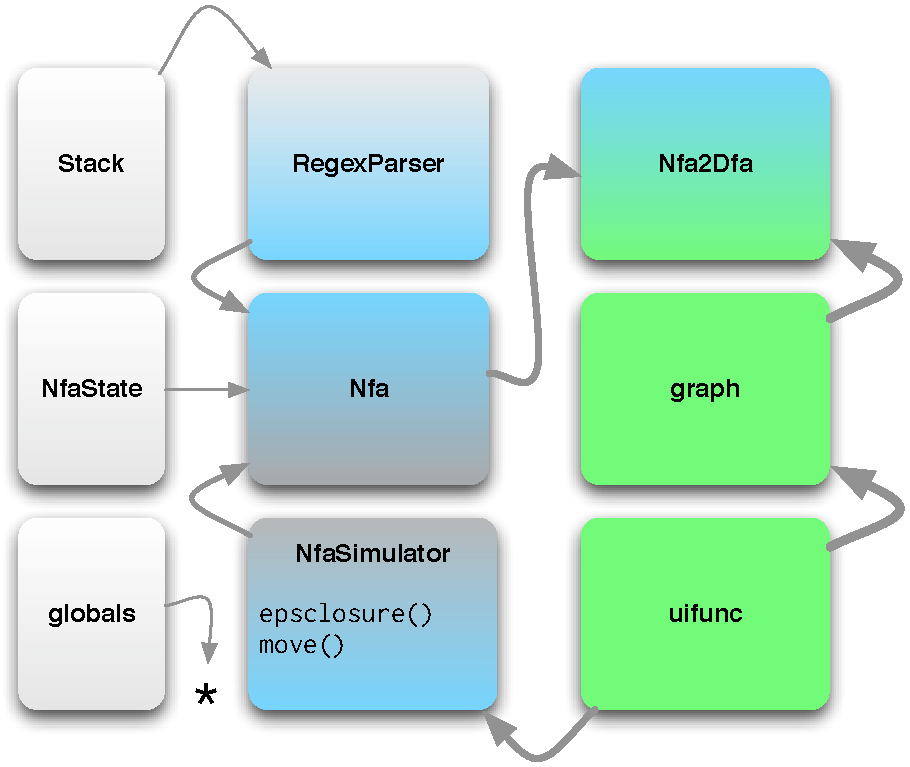
\includegraphics[scale=0.65]{a1.pdf}
            \caption{Konkreter System-Aufbau}
        \end{figure}
    \end{center}
\end{frame}
%%%%%%%%%%%%%%%%%%%%%%%%%%%%%%%%%%%%%%%%%%%%%%%%%%%%%%%%%%%%%%%%%%%%%%%%%%%%%%




%%%%%%%%%%%%%%%%%%%%%%%%%%%%%%%%%%%%%%%%%%%%%%%%%%%%%%%%%%%%%%%%%%%%%%%%%%%%%%
\section{Einfaches Parsing regul"arer Ausdr"ucke}


\subsection{Recursive Descent-Methode}
\begin{frame}[fragile]
    \frametitle{\textit{Recursive Descent}-Methode}

\begin{columns}
    \column{4cm}
    \textbf{Grammatik:}
    \hrule
    \column{7.5cm}
    \textbf{Code:}
    \hrule
\end{columns}

\begin{columns}
    \column{4cm}
    {\scriptsize\begin{tabular}{ll}
        \textbf{expr} & $\rightarrow$ term | term \underline{|} expr \\
        term & $\rightarrow$ factor | term \\
        factor & $\rightarrow$ atom kleene \\
        atom & $\rightarrow$ literal | \underline{(} expr \underline{)}\\
        kleene & $\rightarrow$ \underline{$*$} kleene | $\epsilon$\\
        literal & $\rightarrow$ \underline{a} | \underline{b} | \underline{c} | \underline{\%}
    \end{tabular}}

\column{7.5cm}
\lstset{language=C++, emph={RegexParser}}
\begin{lstlisting}
RegexParser.prototype.expr = function() {
    var nfa = this.term();
    if (this.trymatch('|')) {
        return nfa.union(this.expr());
    };
    return nfa;
};
\end{lstlisting}
\end{columns}

\begin{itemize}
    \item Nahezu direktes "Ubersetzen einer Grammatik\footnote{keine Links-Rekursionen, sonst: Endlosschleife} in den Quelltext des Parsers (LL(1))
    \item $\forall$ Nichtterminale $\exists$ Funktion, welche die rechte Seite der jeweiligen Regel behandelt
    \item Direkte Erzeugung des NDEA, mittels Konstruktion nach Thompson
    \item Max. $2m$ Zust"ande, $4m$ Transitionen ($m$ L"ange des Alphabets)
    %\item Schnell, einfach und effizient
\end{itemize}

\end{frame}


\subsection{Thompson's Algorithmus}
\begin{frame}
    \frametitle{Thompson's Algorithmus}
	
	\begin{itemize}
		\item[{\color{red}Konkatenation: \texttt{ab}}]
\begin{center}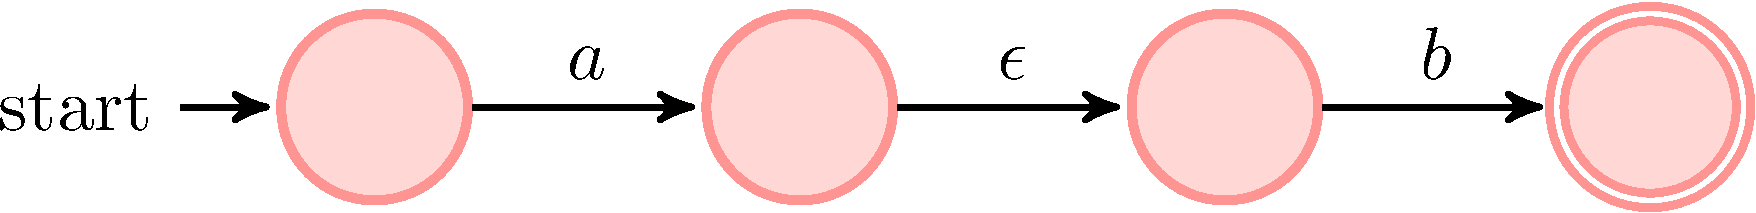
\includegraphics[scale=0.22]{ab.pdf}\end{center}
		\item[]
		\item[{\color{green}H"ulle: \texttt{a*}}]
\begin{center}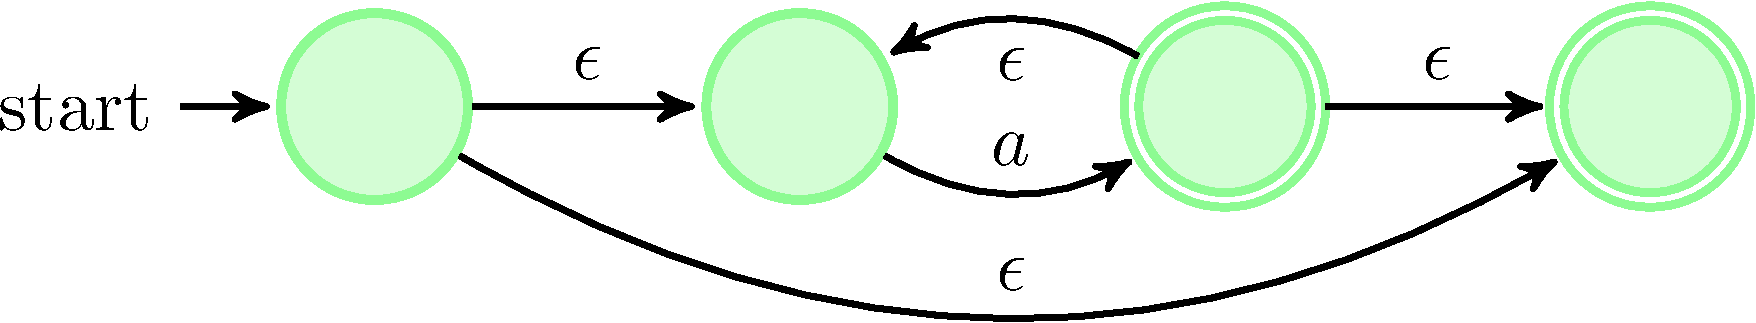
\includegraphics[scale=0.22]{astar.pdf}\end{center}
		\item[]
		\item[{\color{blue}Vereinigung: \texttt{(a|b)}}]
\begin{center}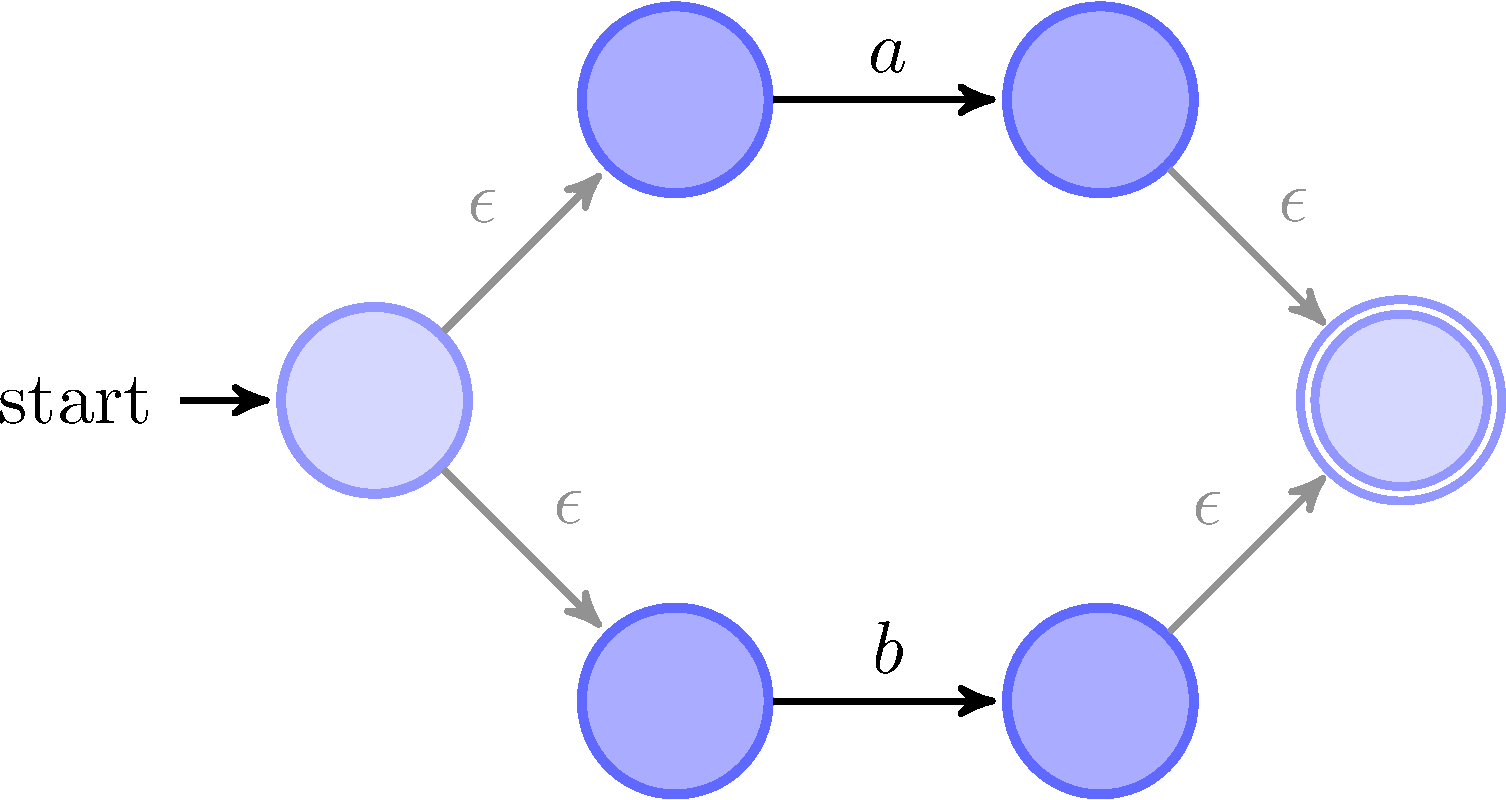
\includegraphics[scale=0.22]{aorb.pdf}\end{center}
	\end{itemize}
\end{frame}


\subsection{Beispiel}
\begin{frame}
    \frametitle{Thompson's Algorithmus: Beispiel}
    
    Regulärer Ausdruck: \texttt{a(a|b)c*}
    \vspace{0.5cm}
	
    \begin{centering}
		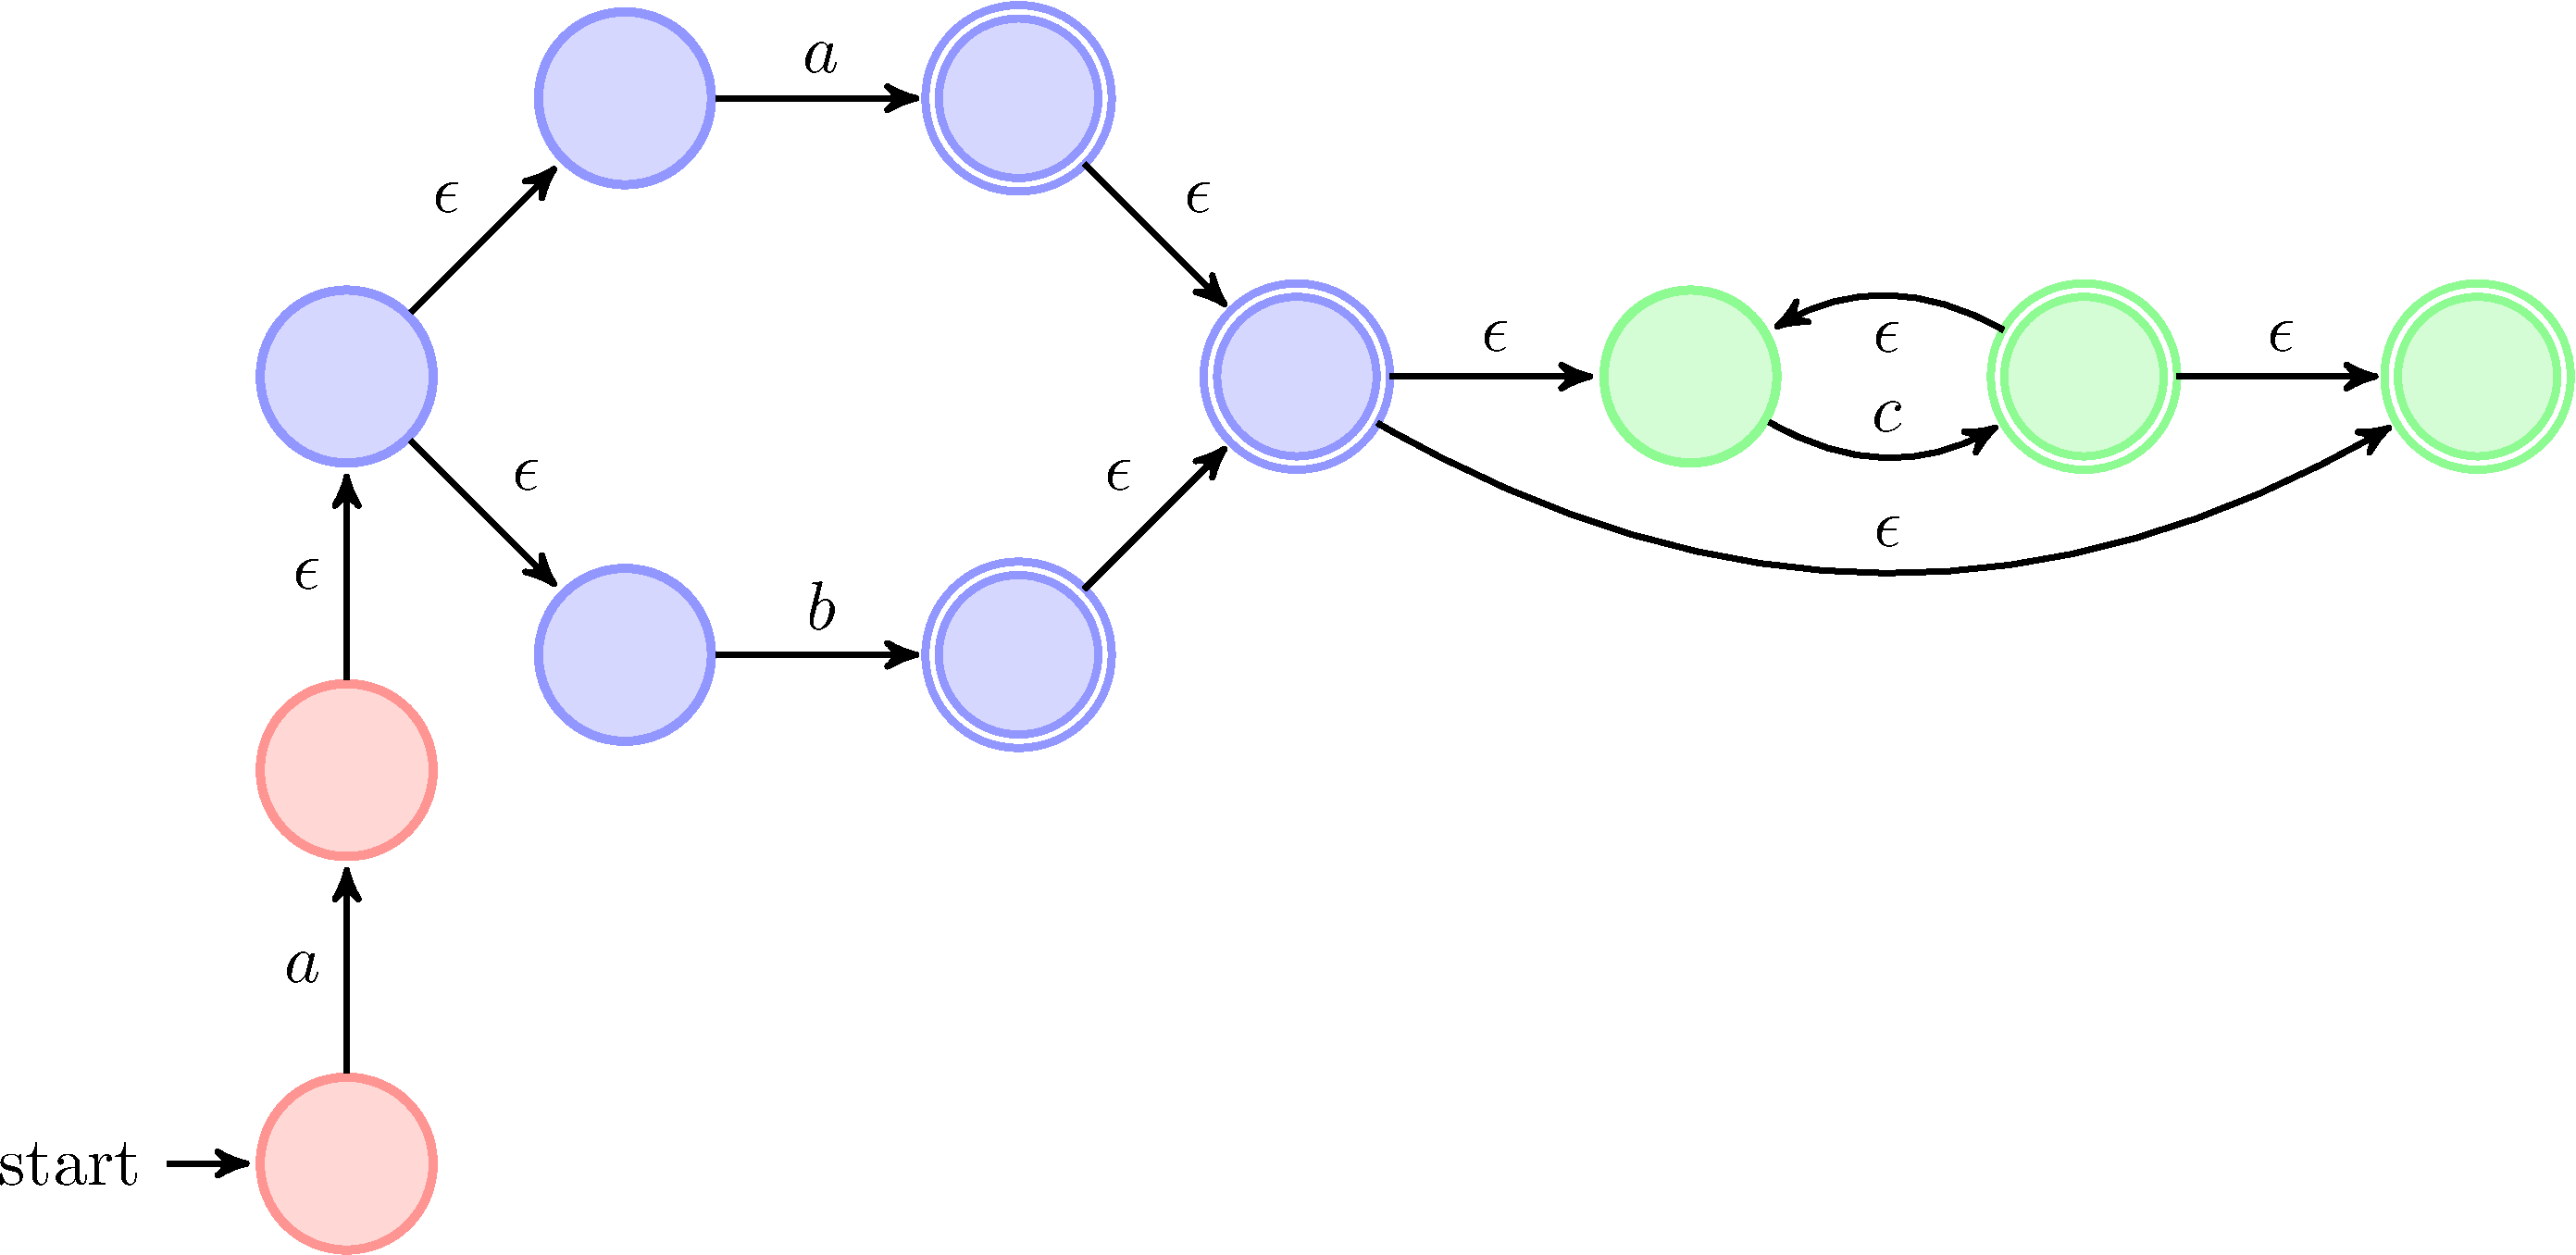
\includegraphics[scale=0.23]{aabc.pdf}
	\end{centering}
\end{frame}
%%%%%%%%%%%%%%%%%%%%%%%%%%%%%%%%%%%%%%%%%%%%%%%%%%%%%%%%%%%%%%%%%%%%%%%%%%%%%%




%%%%%%%%%%%%%%%%%%%%%%%%%%%%%%%%%%%%%%%%%%%%%%%%%%%%%%%%%%%%%%%%%%%%%%%%%%%%%%
\section{"Uberf"uhrung NDEA zu einem DEA}


\subsection*{Einleitung}
\begin{frame}
    \frametitle{Einleitung}

    \begin{itemize}
        \item[] Warum den erzeugten NDEA in einen DEA "uberf"uhren?
        \item[]
        \item \textit{trade-off}:
        \begin{tabular}{rll}
            Platzbedarf & $-$NDEA & \textbf{$\mathbf{+}$DEA}\\
            Erstellungszeit & \textbf{$\mathbf{+}$NDEA} & $-$DEA\\
            Ausf"uhrungszeit & $-$NDEA & \textbf{$\mathbf{+}$DEA}\\
        \end{tabular}
        \item[]
        \item NDEAs\footnote{insbesondere die hier erzeugten} umfassen f"ur gew"ohnlich sehr viele Zust"ande, die Darstellung eines DEA ist praktikabler         
    \end{itemize}

\end{frame}


\subsection{$\epsilon$-Abschluss}
\begin{frame}[fragile]
    \frametitle{$\epsilon$-Abschluss}
    
        \textbf{Pseudo-Code} 
        \hrule
        \begin{columns}
        \column{4.5cm}
\lstset{language=C++, emph={epsclosure,add,move,pop,push,stack,foreach}}
\begin{lstlisting}
epsclosure(dState): stack s
foreach nState in dState {
 s.push(nState)
}
while s not empty { 
 nState1 = s.pop()
 foreach nState1 e> nState2 {
  if nState2 not in dState {
   dState.add(nState2)
   s.push(nState2)
  }
 }
}
return dState
\end{lstlisting}

        \column{4.3cm}
\lstset{language=C++, emph={nfa2dfa,add,DFA,NFA,stack,epsclosure,move,pop,push,foreach}}        
\begin{lstlisting}
nfa2dfa(NFA): stack s, DFA d
s.push(epsclosure(nfa.start))
d.add(epsclosure(nfa.start))
while s not empty {
 dState1 = s.pop()
 foreach ch in ALPHA {
  dState2 = move(dState1, ch)
  next = epsclosure(dState2)
  if next not in DFA {
   d.add(dState ch> next)
  }
 }
}
return d
\end{lstlisting}

        \end{columns}
\begin{itemize}
    \item $\forall p \in Q : E(\{p\}) = \{ q \in Q : p \rightarrow_\epsilon q \}$
    \item \textbf{Laufzeit:} $O(nm^2)$ (bei Vorberechung aller $\epsilon$-Abschl"usse: $O(m)$)  
\end{itemize}
\end{frame}


\subsection{Beispiel}
\begin{frame}[plain]
    \frametitle{NDEA $\rightarrow$ DEA Beispiel}
    
    Regul"arer Ausdruck: \texttt{(a|b)*}

    \begin{center}
        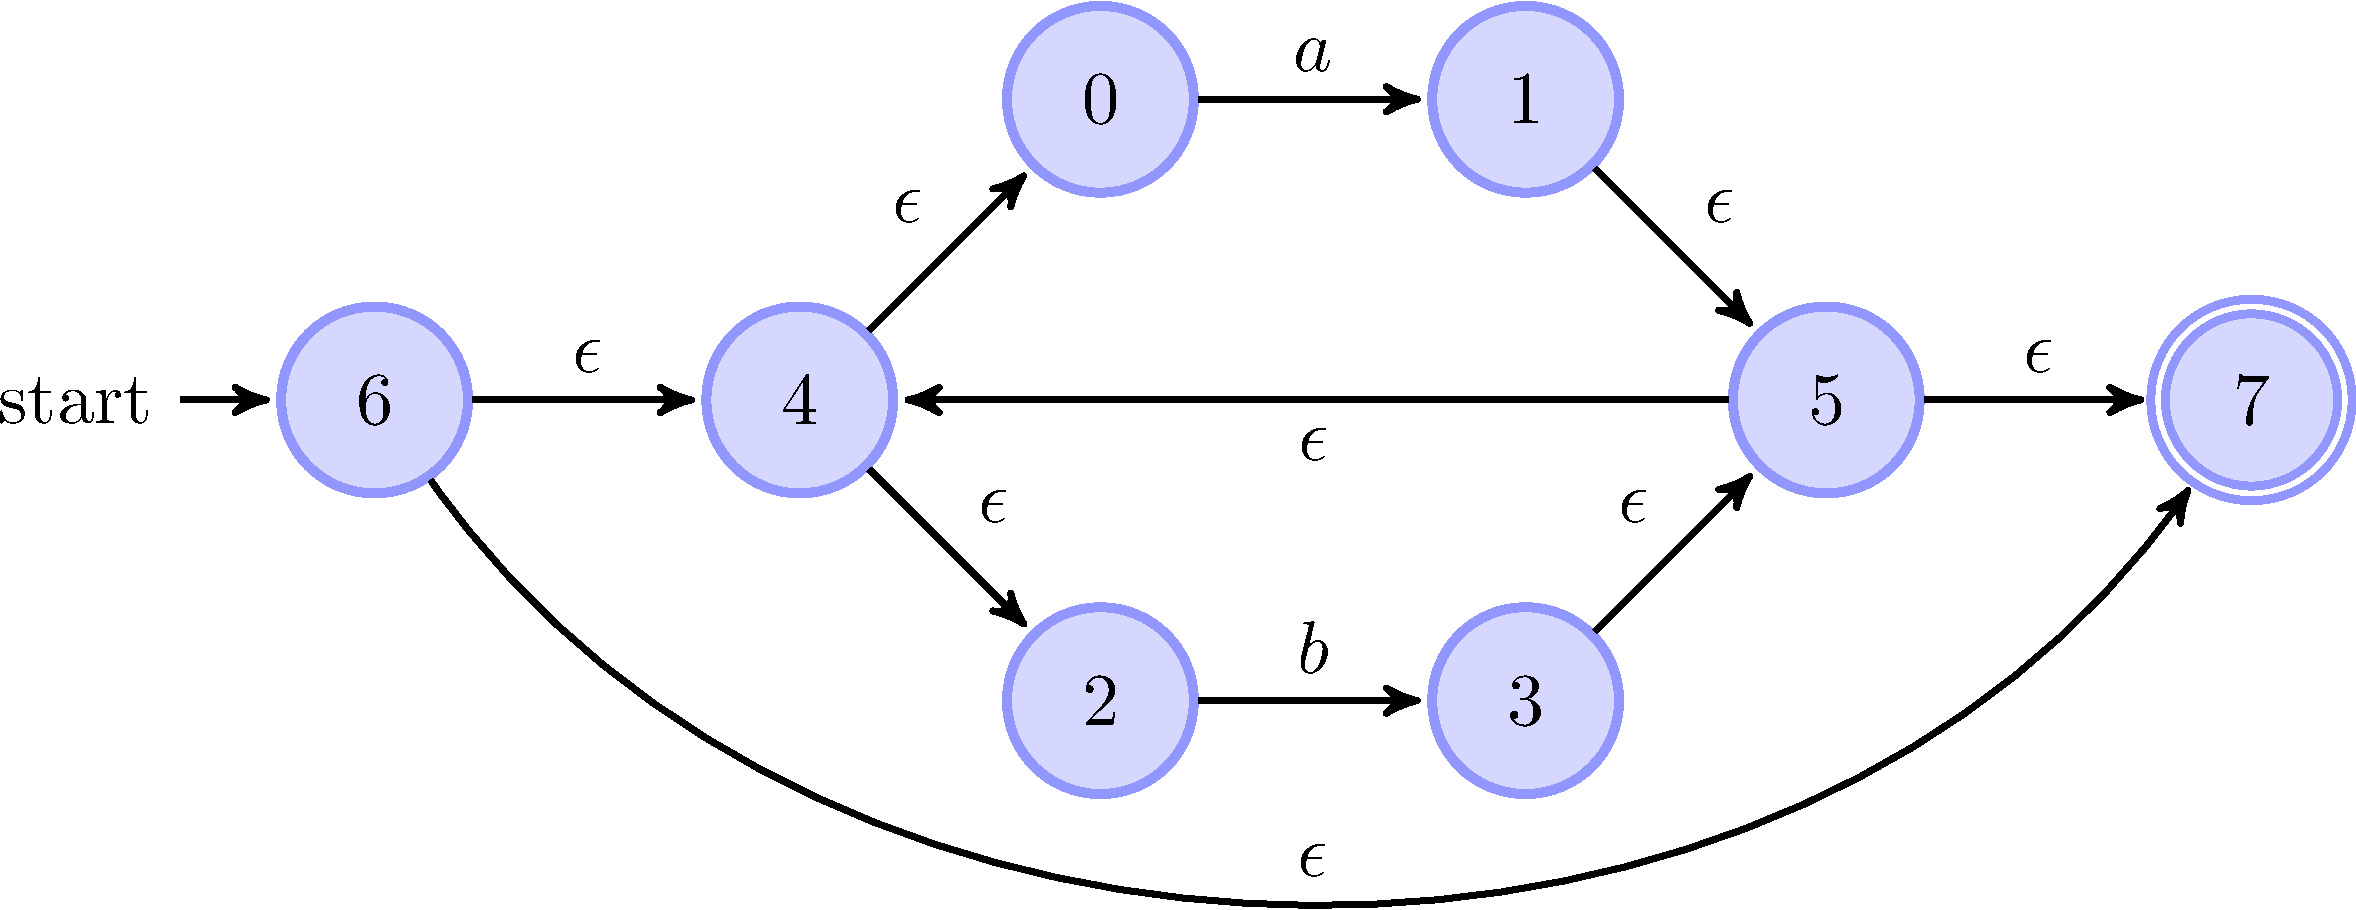
\includegraphics[scale=0.27]{aorbstar0.pdf}
    \end{center}
\end{frame}


\begin{frame}[plain]

\begin{center}
    \frametitle{NDEA $\rightarrow$ DEA Beispiel /2}
    
    \begin{tabular}{c|c|c}
        Dfa ID & Symbol & $\rightarrow$Dfa ID\\
        \hline
        \multirow{2}{*}{\{6, 7, 4, 0, 2\}}   & $a$ & \{1, 5, 7, 4, 0, 2\} \\
                            & $b$ & \{3, 5, 7, 4, 0, 2\} \\
        \hline
        \multirow{2}{*}{\{1, 5, 7, 4, 0, 2\}} & $a$ & \{1, 5, 7, 4, 0, 2\}\\
                             & $b$ & \{3, 5, 7, 4, 0, 2\}\\
        \hline
         \multirow{2}{*}{\{3, 5, 7, 4, 0, 2\}}& $a$ & \{1, 5, 7, 4, 0, 2\}\\
                             & $b$ &  \{3, 5, 7, 4, 0, 2\}\\
    \end{tabular} 
\end{center}

\begin{center}
    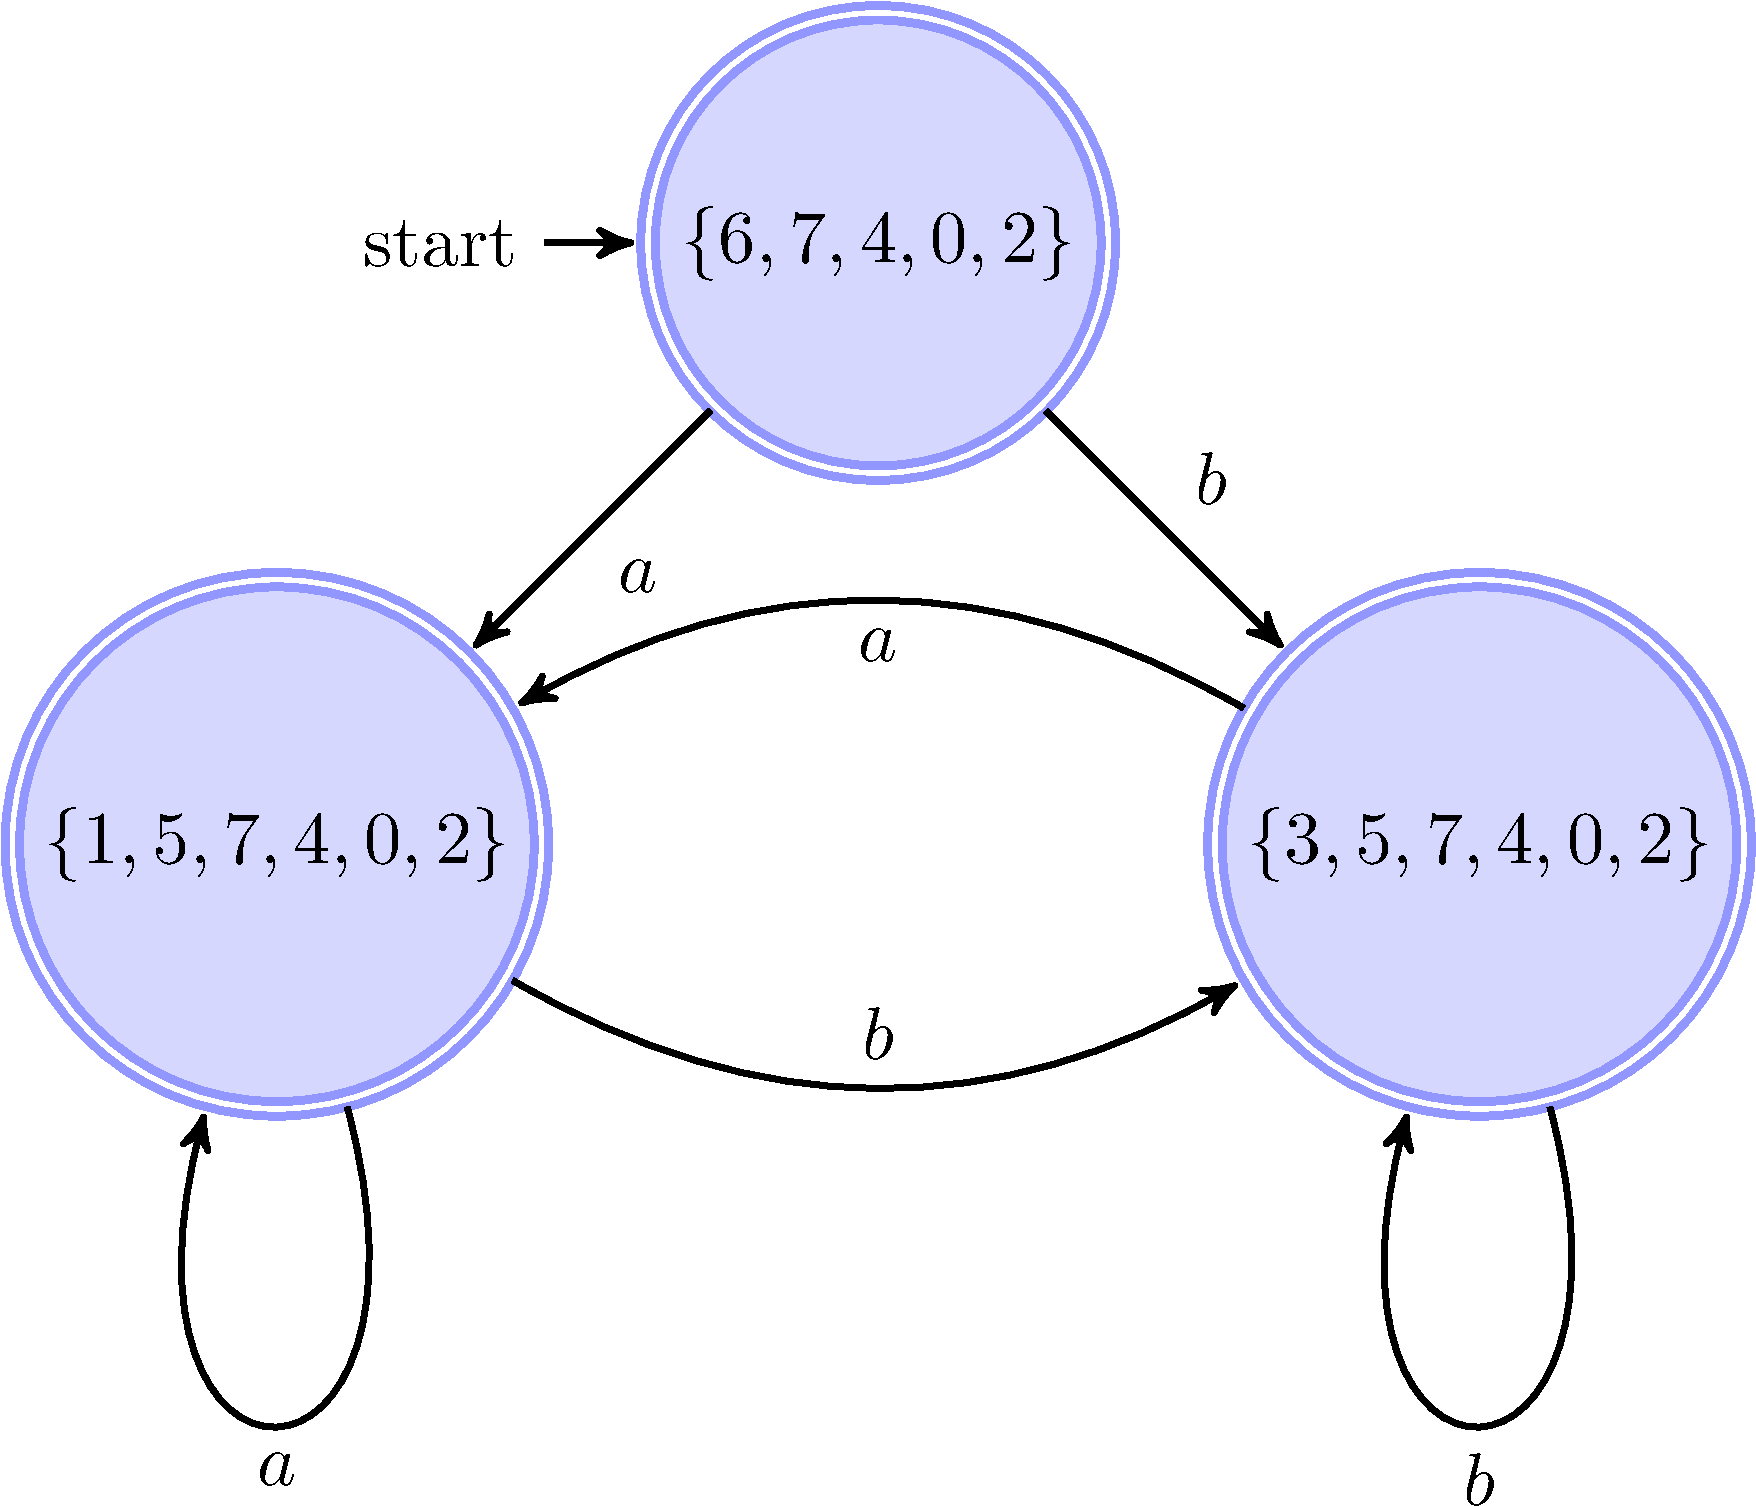
\includegraphics[scale=.175]{aorbstar.pdf}
\end{center}

\end{frame}
%%%%%%%%%%%%%%%%%%%%%%%%%%%%%%%%%%%%%%%%%%%%%%%%%%%%%%%%%%%%%%%%%%%%%%%%%%%%%%


%%%%%%%%%%%%%%%%%%%%%%%%%%%%%%%%%%%%%%%%%%%%%%%%%%%%%%%%%%%%%%%%%%%%%%%%%%%%%%
\begin{frame}[allowframebreaks]
    \frametitle{Literatur}
    \bibliographystyle{alpha}
    \bibliography{beamer}
    \nocite{*}
\end{frame}

\begin{frame}
    \frametitle{Ressourcen}

    \begin{itemize}
        \item \textit{Rapha\"el} JavaScript SVG Library (\url{http://raphaeljs.com/})
        \item \textit{jQuery} JavaScript Library (\url{http://jquery.com/})
        \item Scalable Vector Graphics (\textit{SVG}) 1.1 Specification (\url{http://www.w3.org/TR/SVG/})
        \item Writing your own regular expression parser (\url{http://www.codeproject.com/KB/recipes/OwnRegExpressionsParser.aspx})
    \end{itemize}
\end{frame}
%%%%%%%%%%%%%%%%%%%%%%%%%%%%%%%%%%%%%%%%%%%%%%%%%%%%%%%%%%%%%%%%%%%%%%%%%%%%%%


\section{Demo}
\begin{frame}[plain]
    \begin{center}
        \Huge{Demo}
    \end{center}
\end{frame}


\section{Weiterentwicklung}
\begin{frame}
    \frametitle{Weiterentwicklung}

    \begin{itemize}
        \item Vorhanden: $*$, \texttt{|}, \texttt{()}
        \item[]
        \item Zeichenklassen: \texttt{.}, \texttt{\textbackslash w}, \texttt{\textbackslash d},  \lbrack\ \rbrack, $\hdots$ $\rightarrow$ Einfach implementierbar, Vorverarbeitung der Eingabe
        \item Operatoren: $+$, ?, \{$m$, $n$\}, $\hdots$ $\rightarrow$ Ebenfalls durch Vorverarbeitung l"osbar, beziehungsweise durch Anpassung des Automaten
        \item[]
        \item \textit{Lookahead} oder \textit{lookbehind} sind leider nicht mit endlichen Automaten zu implementieren, da die zugrunde liegenden Grammatiken nicht mehr regul"ar w"aren.
    \end{itemize}
\end{frame}


\end{document}

